\section{Support Vector Machines}
\begin{frame}{The ML Toolbox: Roadmap Update}
    \centering \vspace*{\fill} \hspace*{-0.6cm}
    \resizebox{1.1\linewidth}{!}{
    \begin{tikzpicture}[node distance=0.5cm, box/.style={scale=1.25, rectangle, draw=gray!40, fill=gray!5, rounded corners, minimum width=2.8cm, minimum height=1.8cm, align=center, font=\small}, active/.style={draw=myblue, fill=blue!10, line width=1.5pt}, completed/.style={draw=mygreen, fill=green!10, line width=1pt, dashed}, arrow/.style={-latex, thick, gray!60}]
        \node[font=\bfseries\Large] (root) at (0, 3) {Machine Learning Models ($f_\theta$)};
        \node[box, completed] (linear) at (-6, 0) {\textbf{1. Linear Models}};
        \node[box, completed] (distance) at (-2, 0) {\textbf{2. Distance-Based}};
        \node[box, active] (kernel) at (2, 0) {\textbf{3. Kernel-Based}\\SVM};
        \node[box] (trees) at (6, 0) {\textbf{4. Tree-Based}\\Trees \& Ensembles};
        \draw[arrow] (root) -- (linear); \draw[arrow] (root) -- (distance); \draw[arrow] (root) -- (kernel); \draw[arrow] (root) -- (trees);
        \node[myblue, below=0.3cm of kernel, font=\bfseries] {$\uparrow$ We Are Here};
    \end{tikzpicture}
    } \vspace*{\fill}
\end{frame}

% --- Slide 4: SVM Concept ---
\begin{frame}{Support Vector Machines (SVM)}
    \textit{"Success isn't about barely crossing the line. It's about having some room to spare."}

    \vspace{0.4em}
    Logistic Regression learns a boundary that fits probabilities.
    SVM chooses the boundary with the \textbf{largest safety gap (Margin)}.

    \vspace{0.6em}
    \begin{columns}[c]
        \begin{column}{0.5\textwidth}
            \centering
            \begin{tikzpicture}[scale=0.82]
    \clip (-0.2,-0.6) rectangle (5.4,4.4);

    % ----- Points (now correctly separated) -----
    % Red class (+1): above the upper margin
    \foreach \p in {(1.4,3.9), (1.6,3.7), (1.6,3.95)} \fill[red] \p circle (3pt);
    % Blue class (-1): below the lower margin
    \foreach \p in {(2.3,0.7), (2.4,0.6), (3.0,0.4)} \fill[blue] \p circle (3pt);

    % ----- Decision boundary and margins (all parallel & consistent) -----
    % Boundary: 0.8x + y = 3.8   -> y = -0.8x + 3.8
    \draw[ultra thick] (0,3.8) -- (5,-0.2);

    % Margins: 0.8x + y = 4.4 and 0.8x + y = 3.2
    \draw[dashed, gray!70, thick] (0,4.4) -- (5,0.4);
    \draw[dashed, gray!70, thick] (0,3.2) -- (5,-0.8);

    % ----- Support vectors (on the margins) -----
    \fill[red]  (1.5,3.2) circle (3pt);  % on upper margin (0.8*1.5 + 3.2 = 4.4)
    \draw[red, very thick] (1.5,3.2) circle (6pt);

    \fill[blue] (2.5,1.2) circle (3pt);  % on lower margin (0.8*2.5 + 1.2 = 3.2)
    \draw[blue, very thick] (2.5,1.2) circle (6pt);

    % ----- Margin arrow (between the two dashed lines, along the normal) -----
    \draw[<->, thick, green!60!black]
        (2.2,1.44) -- (3.0,2.0)
        node[(4.0,2.4), above, font=\scriptsize] {Margin};

    % Tiny legend (optional, same as your style)
    \node[font=\scriptsize, align=left] at (3.55,3.75) {
        \textbf{Boundary} (solid)\\
        \textbf{Margins} (dashed)
    };
\end{tikzpicture}

        \end{column}

        \begin{column}{0.5\textwidth}
            \begin{itemize}
                \item \textbf{Hyperplane:} boundary ($\mathbf{w}^T\mathbf{x} + b = 0$).
                \item \textbf{Margin:} “safety gap” to the closest points.
                \item \textbf{Support Vectors:} closest points that \textbf{define} the boundary.
            \end{itemize}

            \vspace{0.4em}
            \begin{tcolorbox}[colback=yellow!10, colframe=orange!70, boxsep=3pt]
                \small Bigger margin $\Rightarrow$ more robust to noise.
            \end{tcolorbox}
        \end{column}
    \end{columns}
\end{frame}

% --- Slide: The Math (Hard Margin) ---
\begin{frame}{Hard Margin SVM}
    We established that we want the \textbf{widest possible margin}.
    Mathematically, maximizing width $\Longleftrightarrow$ minimizing weights $||\mathbf{w}||$.

    \vspace{0.5em}
    \begin{tcolorbox}[colback=white, colframe=black, title=\textbf{The "Hard Margin" Objective}]
        $$ \min_{\mathbf{w}, b} \frac{1}{2} ||\mathbf{w}||^2 $$
        $$ \text{Subject to: } y_i (\mathbf{w}^T \mathbf{x}_i + b) \geq 1 $$
    \end{tcolorbox}

    \vspace{0.5em}
    \begin{tcolorbox}[colback=blue!5, colframe=blue!60, boxsep=4pt]
        \textbf{What does this mean?}
        \begin{itemize}
            \item \textbf{Minimize Objective:} Keep the weights small.
            \item \textbf{Subject to Constraint:} Strictly forbid ANY data point from touching the margin (i.e., being misclassified).
        \end{itemize}
    \end{tcolorbox}
    \centering \footnotesize \textit{*Note: This assumes data is perfectly linearly separable (Hard Margin).}
\end{frame}

% --- Slide: The Reality (Soft Margin) ---
\begin{frame}[allowframebreaks]{Soft Margin: When Perfection is Impossible}
    Real data is noisy (never perfectly linearly separable). A "Hard Margin" would crash if just one outlier existed in the data.
    
    \textbf{Solution:} We relax the rules. We allow some "violations" ($\xi_i$) but penalize them using a hyperparameter \textbf{C}.

    \vspace{0.3em}
    \begin{tcolorbox}[colback=black!3, colframe=black, boxsep=2pt, left=4pt, right=4pt, top=2pt, bottom=2pt]
        \centering \small
        $\displaystyle \min_{\mathbf{w}, b, \boldsymbol{\xi}}\;\; \frac{1}{2}\|\mathbf{w}\|^2 \;+\; \textcolor{red}{\mathbf{C}} \sum_i \xi_i \qquad \text{s.t. } y_i(\mathbf{w}^T\mathbf{x}_i + b) \geq 1 - \xi_i,\;\; \xi_i \geq 0$
        \\[0.2em]
        {\scriptsize \textcolor{red}{$\mathbf{C}$} weights the \emph{total} violation against the margin term, so it shapes \emph{all} the weights $\mathbf{w}$ globally --- not just the outlier points.}
    \end{tcolorbox}
    \framebreak
    \begin{columns}[c]
        \begin{column}{0.5\textwidth}
            \begin{tcolorbox}[colback=red!5, title=\textbf{The Hyperparameter C}]
                \textbf{Large C (Strict)}
                \begin{itemize}
                    \item Penalizes errors heavily.
                    \item Result: Narrow margin, risk of overfitting.
                \end{itemize}
                
                \vspace{0.5em}
                \textbf{Small C (More Violations)}
                \begin{itemize}
                    \item Ignores small errors.
                    \item Result: Wider margin, better generalization.
                \end{itemize}
            \end{tcolorbox}
        \end{column}
        \begin{column}{0.5\textwidth}
            \centering
            % Simple visual of outliers
            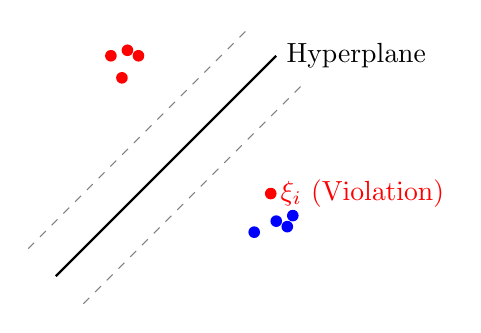
\begin{tikzpicture}[scale=0.7]
                \draw[thick] (0,0) -- (4,4) node[right] {Hyperplane};
                \draw[dashed, gray] (-0.5,0.5) -- (3.5,4.5);
                \draw[dashed, gray] (0.5,-0.5) -- (4.5,3.5);
                
                % Outlier
                \fill[red] (3.9, 1.5) circle (3pt) node[right] {$\xi_i$ (Violation)};
                
                % Normal points
                \fill[blue] (4, 1) circle (3pt);
                \fill[blue] (4.2, 0.9) circle (3pt);
                \fill[blue] (4.3, 1.1) circle (3pt);
                \fill[blue] (3.6, 0.8) circle (3pt);
                \fill[red] (1.5, 4) circle (3pt);
                \fill[red] (1.2, 3.6) circle (3pt);
                \fill[red] (1.3, 4.1) circle (3pt);
                \fill[red] (1, 4) circle (3pt);
            \end{tikzpicture}
            
            \vspace{0.5em}
            \small "Ideally, separate perfectly. If not, minimize the sum of violations."
        \end{column}
    \end{columns}
\end{frame}


% --- Slide: The Kernel Trick ---
\begin{frame}{Handling Non-Linearity: The Kernel Trick}
    \textbf{Problem:} Standard SVM finds a linear boundary. What if data is not linearly separable (e.g., a donut)?
    \pause
    
    \vspace{0.5em}
    \begin{columns}[c]
        \begin{column}{1.0\textwidth}
            \textbf{The Solution (Feature Engineering)}:
            We map inputs to a higher-dimensional space where they \textit{become} separable.
            $$ \mathbf{x} \rightarrow \phi(\mathbf{x}) $$
            (e.g., adding $x^2$ as a new feature).
            \pause
            \vspace{0.3em}

            \textbf{Issue:} Computing $\phi(\mathbf{x})$ explicitly is computationally expensive.
            \pause
            \vspace{0.3em}
            
            \textbf{The "Trick" (Implicit Computation)}:
             We use special type of functions called \textbf{Kernel Functions} which compute the high-dim \textbf{similarity directly} without explicitly building them!
            
            \begin{tcolorbox}[colback=blue!5, colframe=blue!60, boxsep=4pt]
                $$ K(\mathbf{x}_i, \mathbf{x}_j) = \phi(\mathbf{x}_i)^T \phi(\mathbf{x}_j) $$
            \end{tcolorbox}
            \small
            This is called the \textbf{Kernel Trick}.
        \end{column}

        
    \end{columns}
\end{frame}

% --- Slide: Common Kernels ---
\begin{frame}{Common SVM Kernels: A Menu of Similarity}
    The choice of Kernel tells the SVM "how to measure similarity."
    
    \vspace{0.5em}
    \begin{itemize}
        % 1. Linear Kernel
        \item \textbf{1. Linear Kernel} \hfill \textcolor{gray}{\small (Good for Linear Problems)}
        \begin{itemize}
            \item \small $K(\mathbf{x}, \mathbf{y}) = \mathbf{x}^T \mathbf{y}$
            \item \textbf{What it finds:} Straight lines/planes. 
        \end{itemize}
        \vspace{0.5em}

        % 2. Polynomial Kernel
        \item \textbf{2. Polynomial Kernel} \hfill \textcolor{gray}{}
        \begin{itemize}
            \item \small $K(\mathbf{x}, \mathbf{y}) = (\mathbf{x}^T \mathbf{y} + c)^d$
            \item \textbf{What it finds:} Curved boundaries and feature interactions.
        \end{itemize}
        \vspace{0.5em}

        % 3. RBF Kernel
        \item \textbf{3. Radial Basis Function (RBF)} \hfill \textcolor{myblue}{\small (The Default)}
        \begin{itemize}
            \item \small $K(\mathbf{x}, \mathbf{y}) = \exp(-\gamma ||\mathbf{x} - \mathbf{y}||^2)$
            \item \textbf{What it finds:} "Local" similarity. Points are similar only if they are close in distance.
        \end{itemize}
    \end{itemize}

    % Summary Box
    \begin{tcolorbox}[colback=green!5, colframe=green!50!black, boxsep=2pt, left=4pt]
        \textbf{Rule of Thumb:} Start with \textbf{RBF} if you don't know the structure. 
    \end{tcolorbox}
\end{frame}

% % --- Slide 5: SVM Math ---
% \begin{frame}{SVM: The Mathematical Objective}
%     \textbf{Goal: maximize margin} $\;\Longleftrightarrow\;$ Turns out mathematically this is equivalent to \textbf{minimize} $||\mathbf{w}||$!
%     \small (smaller $||\mathbf{w}||$ means a wider margin!).

%     \begin{tcolorbox}[title=\textbf{Hard-Margin SVM (Linearly Separable)}]
%         $$ \min_{\mathbf{w}, b} \frac{1}{2} ||\mathbf{w}||^2 $$
%         $$ \text{Subject to: } y_i (\mathbf{w}^T \mathbf{x}_i + b) \geq 1 \quad \forall i $$
%     \end{tcolorbox}

%     \vspace{0.6em}
%     \begin{tcolorbox}[colback=blue!5, colframe=blue!60, boxsep=3pt]
%     \begin{itemize}
%         \item This is a \textbf{Constrained Optimization} problem: we must minimize an \textbf{objective} (the weights) while satisfying a \textbf{constraint} (the rules).
        
%         \item The constraint here ensures the correct class \textbf{and} enforces a margin of at least one.
        
%         \item Solving this type of optimization problem requires \textbf{Lagrange Multipliers}, which is out of scope for this program.
%     \end{itemize}
% \end{tcolorbox}
% \end{frame}

% % --- Slide 5: SVM Math ---
% \begin{frame}{SVM: The Mathematical Objective}
%     \textbf{Goal: maximize margin} $\;\Longleftrightarrow\;$ Turns out mathematically this is equivalent to \textbf{minimize} $||\mathbf{w}||$!
%     \small (smaller $||\mathbf{w}||$ means a wider margin!).

%     \begin{tcolorbox}[title=\textbf{Hard-Margin SVM (Linearly Separable)}]
%         $$ \min_{\mathbf{w}, b} \frac{1}{2} ||\mathbf{w}||^2 $$
%         $$ \text{Subject to: } y_i (\mathbf{w}^T \mathbf{x}_i + b) \geq 1 \quad \forall i $$
%     \end{tcolorbox}

%     \vspace{0.6em}
%     \begin{tcolorbox}[colback=blue!5, colframe=blue!60, boxsep=3pt]
%     \begin{itemize}
%     \item This is called \textbf{Hard-Margin SVM}, which assumes perfect separation between classes.
%     \item The variant \textbf{Soft-Margin SVM} allows a few "rule breaks" (misclassifications) to improve generalization.
%     \item In practice, this is controlled by the hyperparameter $C$:
%     \begin{itemize}
%         \item \textbf{Small $C$:} Allows more violations (Wider Margin).
%         \item \textbf{Large $C$:} Allows fewer violations (Harder Margin).
%     \end{itemize}
% \end{itemize}
% \end{tcolorbox}
% \end{frame}


% --- Slide 6: SVM Pros/Cons ---
\begin{frame}{SVM: Strengths and Weaknesses}
    \begin{columns}[T]
        \begin{column}{0.48\textwidth}
            \begin{tcolorbox}[colback=green!5, title=\textbf{Advantages}]
                \small
                \begin{itemize}
                    \item \textbf{High Dimensionality:} Works very well when $features \gg samples$.
                    \item \textbf{Powerful:} Different kernels allow for modeling complex non-linear relationships.
                \end{itemize}
            \end{tcolorbox}
        \end{column}
        \begin{column}{0.48\textwidth}
            \begin{tcolorbox}[colback=red!5, title=\textbf{Disadvantages}]
                \small
                \begin{itemize}
                    \item \textbf{Noise Sensitivity:} Sensitive to noise and outliers (if C is large).
                    \item \textbf{Scalability:} Slow for large datasets ($>10k$ samples).
                    \item \textbf{Preprocessing:} Requires feature scaling.
                \end{itemize}
            \end{tcolorbox}
        \end{column}
    \end{columns}
\end{frame}


% ==============================================================================
% SECTION 4: TREE-BASED
% ==============================================================================

\subsection{Tree-Based Models}

% --- Roadmap Update ---
